%TCIDATA{LaTeXparent=0,0,relatorio.tex}



\chapter{Desenvolvimento} \label{chap:Desenvolvimento}

% Resumo opcional. Comentar se não usar.
\resumodocapitulo{``Só sei que nada sei'' -- Sócrates}

\section{Introdução}

Este capítulo apresenta as soluções adotadas para os problemas de planejamento de tarefas e de tomada de decisões, bem como sua modelagem matemática. Nele também são descritos os ambientes de teste em simulação e a modelagem utilizada para descrever o agente móvel. Por último, ainda neste capítulo, é apresentada uma descrição dos testes realizados.

\section{Modelagem Matemática}

Nesta seção são descritas as mudanças realizadas nos modelos matemáticos utilizados nesse projeto. Também é apresentada uma explicação sobre o modelo final do projeto e sobre como as várias teorias se encaixam.

\subsection{Aprendizagem por Reforço para Seleção de Comportamentos} \label{subsection:QLearningSelecaoDeComportamento}

Um comportamento pode ser descrito como um conjunto de reações à estimulos externos, ou seja, ele é um modelo que um agente, ou sistema, utiliza para fazer a escolha de suas ações. Um agente, em um mesmo estado do sistema, pode ter duas escolhas de ação diferentes, se estiver em comportamentos diferentes.

Neste trabalho, a aprendizagem por reforço é utilizada para aprender uma política de seleção de comportamento e não de ações motoras. Para isso, é necessário alterar as equações do algoritmo \textit{Q Learning} para que, ao invés de escolher uma ação $ u \in U $, escolher um comportamento $ b \in B $. Reescrevendo as principais equações desse algoritmo elas são:

\begin{equation} \label{equation:QValueFunctionBehavior}
    Q^t \left( s, b \right) = \int \! \left( r \left( s, b, s' \right) + \gamma \cdot V^{t-1} \left( s' \right) \right) \cdot P \left( s' \mid b, s \right) \, \mathrm{d}s',
\end{equation}

\begin{equation} \label{equation:PolicySelectionBehavior}
    \pi^t \left( s \right) = \underset{b}{argmax} \left( Q^t \left( s, b \right) \right), e
\end{equation}

\begin{equation}
    V^t \left( s \right) = \underset{b}{max} \left( Q^t \left( s, b \right) \right).
\end{equation}

Além disso, as características $ f_j $ agora são ser baseadas em pares estado-comportamento $ \left( S, B \right) $ e não mais em pares estado-ação.

\begin{equation}
	Q \left( S, B \right) = \omega_1 \cdot f_1 \left( S, B \right) + \omega_2 \cdot f_2 \left( S, B \right) + \cdots + \omega_n \cdot f_n \left( S, B \right),
\end{equation}

\begin{equation} \label{equation:QErrorBehavior}
	erro = r \left( s, b, s' \right) + \gamma \cdot \underset{b}{max} \left( Q^{t-1} \left( s', b' \right) \right) - Q^{t-1} \left( s, b \right), e
\end{equation}

\begin{equation} \label{equation:OmegaUpdateBehavior}
	\omega_i^t = \omega_i^{t-1} + \alpha \cdot erro \cdot f_i \left( s, b \right).
\end{equation}


\subsection{Seleção de Comportamentos em um Sistema Parcialmente Observável} \label{subsection:QLearningParcialmenteObservavel}

O algoritmo \textit{Q Learning} foi criado baseado no MDP, que, como citado na seção \ref{section:MDP}, é utilizado para sistemas completamente observáveis%
\footnote{Sistemas em que existe uma função $ f \left( Z \right) $ que, dado uma medida dos sensores, retorna o estado atual do sistema. Em outras palavras, é um sistema em que, dado uma medida $ z \in Z $ dos sensores se sabe, sem dúvidas, qual o estado presente do sistema $ s \in S $%
}. É necessário, então, expandir sua definição para aplicá-lo em um sistema parcialmente observável%
\footnote{Sistema que não é completamente observável, ou seja, que para uma medida $ z \in Z $ dos sensores só se pode estimar qual a probabilidade desse sistema se encontrar num estado $ s \in S $%
}.

Para isso, deve-se primeiramente introduzir uma nova variável $ a \in A $ que representa a distribuição de probabilidades em todos os possíveis estados $ S $. Considere, por exemplo, um caso em que o vetor de estados seja composto por duas variáveis $ S = \binom{S_1}{S_2} $, que podem ter valores $ S_1 \in \left\{1,2,3\right\} $ e $ S_2 \in \left\{verdadeiro, falso\right\} $. Uma variável $ a \in A $, nesse caso, seria dada por cinco variáveis, representando as probabilidades de S ter cada um dos possíveis valores.

$$
	A = \left(
	\begin{matrix}
		P \left( S_1 = 1 \right) & P \left( S_2 = verdadeiro \right) \\
		P \left( S_1 = 2 \right) & P \left( S_2 = falso \right) \\
		P \left( S_1 = 3 \right) &  
	\end{matrix} \right)
$$

A partir dessa definição, utilizando como inspiração o algoritmo POMDP \cite{Thrun:2005:PR:1121596}, o estado $ s \in S $ é substituido, na equação \ref{equation:QValueFunctionQLearning}, por uma variável $ a \in A $, que represente essa distribuição de probabilidades nos possíveis estados $ S $.

\begin{equation} \label{equation:QValueFunctionPartiallyObservable}
    Q^t \left( a, b \right) = \int \! \left( r \left( a, b, a' \right) + \gamma \cdot V^{t-1} \left( a' \right) \right) \cdot P \left( a' \mid b, a \right) \, \mathrm{d}a'.
\end{equation}

Tem-se, agora, uma seleção de política baseada na distribuição de probabilidades nos estados $ s \in S $:

\begin{equation} \label{equation:PolicySelectionPartiallyObservable}
    \pi^t \left( a \right) = \underset{b}{argmax} \left( Q^t \left( a, b \right) \right),
\end{equation}

\begin{equation}
    V^t \left( a \right) = \underset{b}{max} \left( Q^t \left( a, b \right) \right).
\end{equation}


Analogamente às equações \ref{equation:AmostraQLearning} e \ref{equation:QUpdateQLearning} no \textit{Q Learning} original, aprende-se através de amostras obtidas a partir de experiências $ \left( a, b, a', r \right) $.


\begin{equation}
	amostra = r \left( a, b, a' \right) + \gamma \cdot \underset{b}{max} \left( Q^{t-1} \left( a', b' \right) \right),
\end{equation}

\begin{equation}
	Q^t \left( a, b \right) = \left( 1 - \alpha \right) \cdot Q^{t-1} \left( a, b \right) + \alpha \cdot amostra.
\end{equation}

O problema dessa equação é que, ao utilizar um espectro $ a \in A $ de probabilidades de todos os estados $ s \in S $ e não próprio estado, não é possível simplesmente aprender os valores para cada item. Isso acontece pois, mesmo para espaços de estados discretos, há infinitos valores de $ a \in A $ possíveis.

A teoria vista no tópico \ref{subsection:GeneralizaçãoParesEstadoAção} é utilizada, então, para criar uma generalização desses estados através de características deles. Essas características, ao contrário das vistas anteriormente, devem ser baseadas nas probabilidades de se estar/alcançar um estado. Alguns exemplos são:

\begin{itemize}
	\item Distância da posição mais provável do robô, para uma posição que ofereça um produto ( probabilidade de receber uma recompensa * recompensa ) alta;
	\item Distância da posição mais provável do robô, para uma posição que ofereça um produto ( probabilidade de receber uma recompensa * recompensa ) negativa;
	\item Probabilidade de existir algum perigo (recompensa negativa) a menos que uma certa distância;
	\item Probabilidade de capturar um alvo;
	\item Porcentagem de chance do robô ter um erro.
\end{itemize}

Essas características podem, como no caso anterior, descrever também o comportamento a ser executado, como:

\begin{itemize}
	\item Tentar capturar um alvo;
	\item Tentar fugir de um perigo;
	\item Economizar energia.
\end{itemize}

Com isso um valor $ Q \left( A, B \right) $ é obtido, tal como descrito na equação \ref{equation:QValueFinal1}.

\begin{equation} \label{equation:QValueFinal1}
	Q \left( A, B \right) = \omega_1 \cdot f_1 \left( A, B \right) + \omega_2 \cdot f_2 \left( A, B \right) + \cdots + \omega_n \cdot f_n \left( A, B \right).
\end{equation}


Com esse novo modelo, é possível aprender valores, a partir de cada experiência, utilizando o erro atual do sistema:

\begin{equation} \label{equation:ErroQPartiallyObservable}
	erro = r \left( a, b, a' \right) + \gamma \cdot \underset{b}{max} \left( Q^{t-1} \left( a', b' \right) \right) - Q^{t-1} \left( a, b \right).
\end{equation}
e o utilizando para atualizar cada um dos pesos usados para obter $ Q^t \left( A, B \right) $:
\begin{equation} \label{equation:UpdateOmegaQPartiallyObservable}
	\omega_i^t = \omega_i^{t-1} + \alpha \cdot erro \cdot f_i \left( a, b \right).
\end{equation}

Assim, caso exista um erro grande para um dado espectro de probabilidades, são atualizados os valores de todos os casos que possuam espectros de probabilidades dos estados com características similares àquele. E caso esse estado tenha um valor maior para uma das características, o peso dela será mais modificado que as outras.

Então, caso for utilizada como característica, por exemplo, $ f_i = $ ``probabilidade de existir algum perigo (recompensa negativa) a menos que uma certa distância''. Se for recebida uma recompensa negativa em um estado no qual o valor de $ f_i $ é alto, estados com essa característica serão considerados piores. Se for recebida uma recompensa positiva, os estados com valor alto para essa característica serão considerados melhores.


\subsection{Abordagem Bayesiana com a Seleção de Comportamentos} \label{subsection:BayesComSelecaoDeComportamento}

Partindo dos modelos obtidos na seção \ref{section:FiltroBayesiano}, pode-se agora utilizar a seleção de comportamento, vista no tópico \ref{subsection:QLearningParcialmenteObservavel}, como uma nova medida de sensor, fazendo:

\begin{equation}
	Z' = \binom{Z}{Z_b} = \binom{Z}{B}.
\end{equation}

Sendo $ Z $ as medidas sensorias e $ B = Z_b $ o comportamento obtido utilizando a aprendizagem por reforço. É necessário expandir também o modelo dos estados para:

\begin{equation}
	S' = \binom{S}{S_b}
\end{equation}

Sendo, novamente, $ S $ o modelo do estado atual usual e $ S_b $ uma variável de estado que representa o comportamento atual do agente.

O filtro bayesiano é, então, reescrito como:

\begin{equation}
        P \left( M^{0: t} S^{0: t} S_b^{0: t} Z^{0: t} B^{0: t} \mid \pi_f \right) = P \left( M^0 S^0 S_b^0 Z^0 B^0 \mid \pi_f \right) \cdot \prod\limits_{j =1}^{t} 
        \left(
            \begin{array}{l}
                P \left( S^j S_b^j \mid S^{j -1} S_b^{j-1} M^{j -1} \pi_f \right) \\
                \times P \left( Z^j B^j \mid S^j S_b^{j-1} \pi_f \right) \\
                \times P \left( M^j \mid S^j S_b^j M^{j -1} \pi_f \right)
            \end{array}
        \right).
\end{equation}

Existem três etapas para atualizar o estado $ S'^t $ recursivamente. Para esse novo filtro elas são:

\begin{itemize}
	\item Predição:
		\begin{equation}
    P \left( S^t S_b^t \mid z^{0: t-1} b^{0: t-1} m^{0: t-1} \pi_f \right) \propto \sum\limits_{S^{t-1} S_b^{t-1}}
        \left(
            \begin{array}{l}
                P \left( S^t S_b^t \mid S^{t-1} S_b^{t-1}  m^{t-1} \pi_f \right) \\
                \times P \left( m^{t-1} \mid S^{t-1} S_b^{t-1} m^{t-2} \pi_f \right)\\
                \times P \left( S^{t-1} S_b^{t-1} \mid z^{0: t-1} b^{0: t-1} m^{0: t-2} \pi_f \right)
            \end{array}
        \right);
		\end{equation}
	\item Observação:
		\begin{equation}
    P \left( S^t S_b^t \mid z^{0: t} b^{0: t} m^{0: t-1} \pi_f \right) \propto
        \left(
            \begin{array}{l}
                P \left( z^t b^t \mid S^t S_b^t \pi_f \right) \\
                \times P \left( S^t S_b^t \mid z^{0: t-1} b^{0: t-1} m^{0: t-1} \pi_f \right)
            \end{array}
        \right);
		\end{equation}
	\item Seleção de ação motora:
		\begin{equation}
    P \left( M^t \mid z^{0: t} b^{0: t} m^{0: t-1} \pi_f \right) \propto \sum\limits_{S_i^{t-1} S_b^{t-1}}
        \left(
            \begin{array}{l}
                P \left( M^t \mid S^t S_b^t m^{t-1} \pi_f \right)\\
                \times P \left( S^t S_b^t \mid z^{0: t} b^{0: t} m^{0: t-1} \pi_f \right)
            \end{array}
        \right).
		\end{equation}
\end{itemize}

Assume-se que o estado $ S^t $ é independente do comportamento sendo executado no mesmo momento $ S_b^t $ e que esse comportamento atual independe de tempos anteriores. Assume-se, também, que os dados sensoriais $ Z^t $ são independentes do comportamento escolhido pelo \textit{Q Learning} ($ B^t $) num mesmo momento. Com isso, é possível simplificar o filtro para:

\begin{equation}
	\begin{split}
        P \left( M^{0: t} S^{0: t} S_b^{0: t} Z^{0: t} B^{0: t} \mid \pi_f \right) = \\
        		P \left( M^0 S^0 S_b^0 Z^0 B^0 \mid \pi_f \right) \cdot \prod\limits_{j =1}^{t} 
        &\left(
            \begin{array}{l}
                P \left( S^j \mid S^{j -1} M^{j -1} \pi_f \right) \times P \left( S_b^j \mid \pi_f \right) \\
                \times P \left( Z^j \mid S^j \pi_f \right) \times P \left( B^j \mid S_b^{j-1} \pi_f \right) \\
                \times P \left( M^j \mid S^j S_b^j M^{j -1} \pi_f \right)
            \end{array}
        \right).
	\end{split}
\end{equation}


Pode-se perceber que o modelo de seleção de ação motora:
\begin{equation}
	P \left( M^t \mid S^t S_b^t M^{t-1} \pi_f \right),
\end{equation}
agora depende do comportamento sendo utilizado.

\begin{equation}
    P \left( M^t \mid S^t S_b^t M^{t-1} \pi_f \right) = 
        \left\{
            \begin{array}{l}
                P \left( M^t \mid S^t \left[ S_b^t=b_1 \right] M^{t-1} \pi \right) \\
                P \left( M^t \mid S^t \left[ S_b^t=b_2 \right] M^{t-1} \pi \right) \\
                \cdots \\
                P \left( M^t \mid S^t \left[ S_b^t=b_{N_b} \right] M^{t-1} \pi \right)
            \end{array}.
        \right.
\end{equation}

A vantagem é que pode-se ter, para cada comportamento, um modelo de ação diferente. Esse modelo pode ainda ser escrito em sua forma recursiva, para um dado instante de tempo $ t $, ficando como na equação \ref{equation:BayesianModelFinalRecursivo}.
\begin{equation} \label{equation:BayesianModelFinalRecursivo}
	\begin{split}
        P \left( M^{0: t} S^{0: t} S_b^{0: t} Z^{0: t} B^{0: t} \mid \pi_f \right) = \\
        		P \left( M^{0: t-1} S^{0: t-1} S_b^{0: t-1} Z^{0: t-1} B^{0: t-1} \mid \pi_f \right) \cdot 
        &\left(
            \begin{array}{l}
                P \left( S^t \mid S^{t -1} M^{t -1} \pi_f \right) \times P \left( S_b^t \mid \pi_f \right) \\
                \times P \left( Z^t \mid S^t \pi_f \right) \times P \left( B^t \mid S_b^{t-1} \pi_f \right) \\
                \times P \left( M^t \mid S^t S_b^t M^{t -1} \pi_f \right)
            \end{array}
        \right).
	\end{split}
\end{equation}

Esse filtro simplificado pode, como o na seção \ref{section:FiltroBayesiano}, ser escrito na sua forma recursiva e separado em 3 etapas.

\begin{itemize}
	\item Predição:
		\begin{equation}
    P \left( S^t S_b^t \mid z^{0: t-1} b^{0: t-1} m^{0: t-1} \pi_f \right) \propto \sum\limits_{S^{t-1} S_b^{t-1}}
        \left(
            \begin{array}{l}
                P \left( S^t \mid S^{t-1} m^{t-1} \pi_f \right) \times P \left( S_b^t \mid \pi_f \right) \\
                \times P \left( m^{t-1} \mid S^{t-1} S_b^{t-1} m^{t-2} \pi_f \right)\\
                \times P \left( S^{t-1} S_b^{t-1} \mid z^{0: t-1} b^{0: t-1} m^{0: t-2} \pi_f \right)
            \end{array}
        \right);
		\end{equation}
	\item Observação:
		\begin{equation}
    P \left( S^t S_b^t \mid z^{0: t} b^{0: t} m^{0: t-1} \pi_f \right) \propto
        \left(
            \begin{array}{l}
                P \left( z^t \mid S^t \pi_f \right) \times P \left( b^t \mid S_b^t \pi_f \right) \\
                \times P \left( S^t S_b^t \mid z^{0: t-1} b^{0: t-1} m^{0: t-1} \pi_f \right)
            \end{array}
        \right);
		\end{equation}
	\item Seleção de ação motora:
		\begin{equation}
    P \left( M^t \mid z^{0: t} b^{0: t} m^{0: t-1} \pi_f \right) \propto \sum\limits_{S^{t-1} S_b^{t-1}}
        \left(
            \begin{array}{l}
                P \left( M^t \mid S^t S_b^t m^{t-1} \pi_f \right)\\
                \times P \left( S^t S_b^t \mid z^{0: t} b^{0: t} m^{0: t-1} \pi_f \right)
            \end{array}
        \right).
		\end{equation}
\end{itemize}


\subsection{Modelo Final e Completo}

Em posse da modelagem matemática introduzida no capítulo \ref{chap:FundamentacaoMatematica} e explorada nos tópicos \ref{subsection:QLearningSelecaoDeComportamento}, \ref{subsection:QLearningParcialmenteObservavel} e \ref{subsection:BayesComSelecaoDeComportamento} é possível agora apresentar o modelo completo utilizado neste trabalho.

É possível separar esse modelo em duas partes: uma de treinamento e outra em que a aprendizagem já foi comcluída.

Durante a fase de treinamento, então, um modelo com cinco etapas é utilizado. As já conhecidas: predição; observação; seleção de ação motora. Integradas com a seleção de comportamento e aprendizagem. Esse modelo está representado na figura \ref{img:ModeloFinalTreinamento}.

\begin{figure}[H]
    \centering
    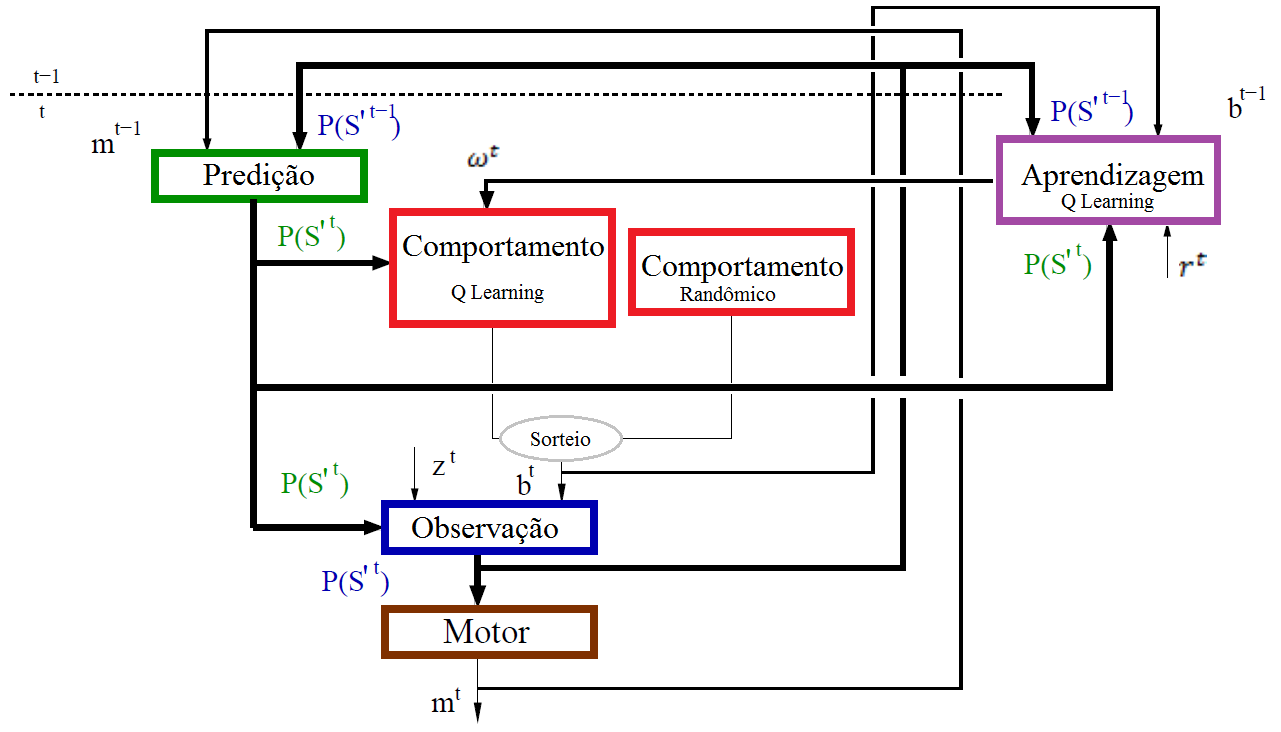
\includegraphics[width=150mm]{images/modelo_bayesiano_treino-tiago}
    \caption{Filtro Bayesiano utilizando \textit{Q Learning} para Seleção de Comportamento. Durante treinamento.}
    \label{img:ModeloFinalTreinamento}
\end{figure}

Após acabado o treinamento, não se tem mais necessidade da etapa de aprendizagem, ficando então um modelo com apenas 4 etapas. Esse modelo pode ser representado pela figura \ref{img:ModeloFinalPosTreinamento}.

\begin{figure}[h!]
    \centering
    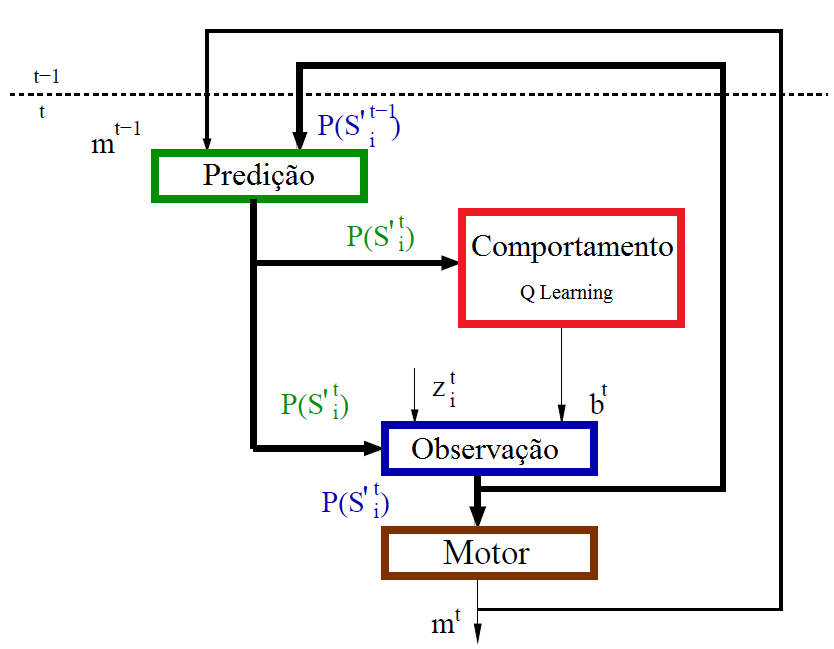
\includegraphics[width=120mm]{images/modelo_bayesiano_final-tiago}
    \caption{Filtro Bayesiano utilizando \textit{Q Learning} para Seleção de Comportamento. Após treinamento completo.}
    \label{img:ModeloFinalPosTreinamento}
\end{figure}

\subsubsection{Predição} \label{subsubsection:ModeloFinalPredicao}

Nessa etapa, a partir da ação escolhida no período anterior de tempo (instante de tempo $ t-1 $), se faz uma estimativa de qual será o estado após sua execução (instante de tempo $ t $).

\begin{equation}
    P \left( S^t S_b^t \mid z^{0: t-1} b^{0: t-1} m^{0: t-1} \pi_f \right) \propto \sum\limits_{S^{t-1} S_b^{t-1}}
        \left(
            \begin{array}{l}
                P \left( S^t \mid S^{t-1} m^{t-1} \pi_f \right) \times P \left( S_b^t \mid \pi_f \right) \\
                \times P \left( m^{t-1} \mid S^{t-1} S_b^{t-1} m^{t-2} \pi_f \right)\\
                \times P \left( S^{t-1} S_b^{t-1} \mid z^{0: t-1} b^{0: t-1} m^{0: t-2} \pi_f \right)
            \end{array}
        \right).
\end{equation}


\subsubsection{Escolha de comportamento}

Essa etapa é onde a escolha do comportamento acontece. Ela pode ter dois métodos distintos, um durante a fase de treinamento e outro após acabar a aprendizagem.

Durante a aprendizagem se utiliza uma exploração gulosa, descrita no tópico \ref{subsection:EscolhaDeAçõesExploraçãoGulosa}, para fazer essa escolha do comportamento. Nela, primeiro se sorteia um número randômico $ x \in [0,1] $. Se esse número for menor que um fator de exploração $ \gamma $, se escolhe um comportamento randômico entre todos os possíveis. No caso contrário, se escolhe um comportamento da mesma forma que após a aprendizagem ter acabado, descrito a seguir.

Para a escolha de comportamento após terminado o treinamento, primeiro se calcula a função \ref{equation:QLearningEscolhaComportamentoFinal}, à seguir, para cada comportamento $ b \in B^t $ e para o conjunto de probabilidades%
\footnote{É importante ressaltar que $ a^t $ equivale ao conjunto de probabilidades $ P \left( S^t S_b^t \mid z^{0: t-1} b^{0: t-1} m^{0: t-1} \pi_f \right) $, obtido em \ref{subsubsection:ModeloFinalPredicao}.%
} $ a^t \in A^t $ de se encontrar em cada estado $ S^t $.

\begin{equation} \label{equation:QLearningEscolhaComportamentoFinal}
    	Q \left( a^t, B^t \right) = \omega^1 \cdot f^1 \left( a^t, B^t \right) + \omega^2 \cdot f^2 \left( a^t, B^t \right) + \cdots + \omega^n \cdot f^n \left( a^t, B^t \right)
\end{equation}

Depois, se escolhe um comportamento a partir desses valores calculados, sendo escolhido o que maximiza essa função.


\subsubsection{Observação}

A partir dos sensores presentes no robô e do valor $ b \in B $, obtido com o algoritmo de aprendizado, se atualiza o estado probabilístico (\textit{belief state}) do agente.

\begin{equation}
    P \left( S^t S_b^t \mid z^{0: t} b^{0: t} m^{0: t-1} \pi_f \right) \propto
        \left(
            \begin{array}{l}
                P \left( z^t \mid S^t \pi_f \right) \times P \left( b^t \mid S_b^t \pi_f \right) \\
                \times P \left( S^t S_b^t \mid z^{0: t-1} b^{0: t-1} m^{0: t-1} \pi_f \right)
            \end{array}
        \right).
\end{equation}


\subsubsection{Escolha de ação motora}

Por último se faz a seleção de uma ação a ser executada pelo robô. Para isso, calcula-se a distribuição de probabilidade de se executar cada ação $ m^t \in M^t $ e se escolhe a ação que possui maior valor nessa distribuição.

\begin{equation}
    P \left( M^t \mid z^{0: t} b^{0: t} m^{0: t-1} \pi_f \right) \propto \sum\limits_{S^t S_b^t}
        \left(
            \begin{array}{l}
                P \left( M^t \mid S^t S_b^t m^{t-1} \pi_f \right)\\
                \times P \left( S^t S_b^t \mid z^{0: t} b^{0: t} m^{0: t-1} \pi_f \right)
            \end{array}
        \right)
\end{equation}


\subsubsection{Aprendizagem}

Nessa etapa são atualizados os valores do modelo de seleção de comportamento $ Q \left( A, B \right) $ a partir de uma recompensa $ r $ recebida. Tendo posse dessa recompensa, da distribuição de probabilidades do estado anterior $ a^{t-1} \in A^{t-1} $ e atual $ a^t \in A^t $ do sistema e de qual o comportamento $ b^{t-1} \in B^{t-1} $ escolhido no tempo anterior pelo algoritmo de aprendizagem, é possível atualizar os pesos $ \omega_i $ do sistema de aprendizagem, como descrito nas equações \ref{equation:ErroQPartiallyObservable} e \ref{equation:UpdateOmegaQPartiallyObservable}, reescritas aqui por conveniência.

$$
	erro = r \left( a, b, a' \right) + \gamma \cdot \underset{b}{max} \left( Q^{t-1} \left( a', b' \right) \right) - Q^{t-1} \left( a, b \right)
$$

$$
	\omega_i^t = \omega_i^{t-1} + \alpha \cdot erro \cdot f_i \left( a, b \right)
$$



\section{Ambiente de Testes e Simulação} \label{section:AmbienteDeTestes}

Para poder testar as teorias aqui descritas foi utilizado uma plataforma de Pacman%
\footnote{Essa plataforma pode ser encontrada em http://ai.berkeley.edu/project\_overview.html%
}, criada em Berkeley para suas aulas de inteligência artificial.

\begin{figure}[h]
    \centering
    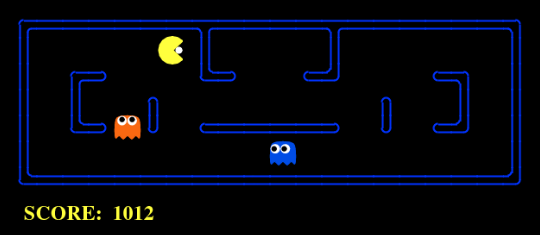
\includegraphics[width=120mm]{images/pacman_platform}
    \caption{\label{img:PlataformaSimulacaoPacman}Plataforma do jogo Pacman desenvolvida em Berkeley para aulas de IA.}
\end{figure}

A plataforma provê um sistema com informação completa%
\footnote{Todas as propriedades do jogo são conhecidas a todo momento, como por exemplo: posição do Pacman, posição dos fantasmas e localizações com ou se comida.%
} e sem erros na movimentação%
\footnote{Uma ação executada em um dado estado do sistema terá sempre o mesmo resultado.%
}. Essa plataforma foi programada em python e integrada com ROS \cite{ROS:1448}. Utilizando o ROS essa plataforma foi conectada com um programa em C++, no qual foi programado o modelo de aprendizagem e seleção de comportamento proposto neste trabalho.

A comunicação entre a plataforma em Python e o programa em C++ se dá a partir de quatro mensagens diferentes, as quais simulam os sensores, atuadores e recompensas do sistema.

\begin{itemize}
	\item Posição do agente (Pacman) --- $ \left( x, y \right) \in \mathbb{R}^2 $;
	\item Distância para os fantasmas --- $ \left( d_x, d_y \right) = \left( \Delta x, \Delta y \right) \in \mathbb{R}^2 $;
	\item Ação a ser executada --- $ u \in \left\{Norte, Sul, Leste, Oeste, Esperar \right\} $;
	\item Recompensa recebida do ambiente --- $ r \in \mathbb{R} $.
\end{itemize}

Para simular erros de sensoriamento, comuns em aplicações de robótica móvel, antes de enviar essas informações são inseridos erros Gaussianos tanto na posição do agente (Pacman), quanto nas distâncias para os fantasmas.

$$
	\left( x, y \right) = \left( x^*, y^* \right) + \left( \delta\left( 0, \sigma_{pacman} \right), \delta\left( 0, \sigma_{pacman} \right) \right),
$$

\begin{equation}
	\left( x, y \right) = \left( \delta\left( x^*, \sigma_{pacman} \right), \delta\left( y^*, \sigma_{pacman} \right) \right).
\end{equation}

Sendo:

\begin{itemize}
	\item $ \delta \left( \mu, \sigma \right) $ uma função que gera um número aleatório baseado numa gaussiana com média $ \mu $ e desvio padrão $ 
sigma $;
	\item $ \sigma_{pacman} $ o desvio padrão do erro inserido na posição do agente;
	\item $ \left( x^*, y^* \right) $ a posição exata do agente.
\end{itemize}

Analogamente a distância percebida para os fantasmas é:

\begin{equation}
	\left( d_x, d_y \right) = \left( \delta\left( d_x^*, \sigma_{dist\_fant} \right), \delta\left( d_y^*, \sigma_{dist\_fant} \right) \right).
\end{equation}

A atuação tem um conjunto de valores possível tal que $ u \in U = \{ Norte,\allowbreak Sul,\allowbreak Leste,\allowbreak Oeste,\allowbreak Parar \} $. Por ela possuir um valor discreto e não numérico, não se insere um erro gaussiano gaussiano nela. Para simular erros de atuação, quando uma ação é recebida pela plataforma de simulação ela é executada de acordo com a função prensente no algorítmo \ref{algorithm:ErroAtuacao}.

\begin{algorithm}[h]
	\caption{Erro na Atuação} \label{algorithm:ErroAtuacao}
	\begin{algorithmic}[1]
		\Procedure{Executar\_Ação}{\textit{ação\_escolhida}}
			\State $\textit{numero\_randomico} \gets \text{random }\textit{numero}$
			\If {$\textit{numero\_randomico} > \text{FATOR\_DE\_ACERTO} $ }
				\State $\textit{acao\_randomica} \gets \text{random }\textit{ação} \in \textit{Ações}-\textit{\{ação\_escolhida\}}$
				\State \Return $\textit{acao\_randomica}$
			\Else
				\State \Return $\textit{ação\_escolhida}$
			\EndIf
		\EndProcedure
	\end{algorithmic}
\end{algorithm}

Ou seja, a atuação tem uma chance $ \nu_{atuacao} = \textit{FATOR\_DE\_ACERTO} $ de ser executada como esperado. Existe também uma proabilidade $ 1 - \nu_{atuacao} $ de ser selecionada uma ação randômica diferente da escolhida.

A recompensa $ r $ é, por sua vez, enviada da plataforma de simulação para o sistema de aprendizagem. Nela não é inserida qualquer forma de erro e ela representa a diferença de pontuação entre a etapa atual e a anterior no jogo, ou seja, a pontuação recebida pela última ação executada.


\section{Testes Realizados} \label{section:TestesRealizados}

Nessa seção é apresentado o setup de cada teste realizado e analisado no capitulo \ref{chap:Resultados}, além dos parâmetros utilizados.

\subsection{3 Comportamentos no mapa pequeno (Teste 1)} \label{subsection:3ComportamentosMapaPequeno}

Esse primeiro teste foi feito no mapa pequeno, mostrado na figura \ref{img:PlataformaPacmanMapaPequeno}, e foram utilizados apenas três comportamentos:

\begin{itemize}
	\item Parar;
	\item Comer;
	\item Fugir.
\end{itemize}

\begin{figure}[h]
    \centering
    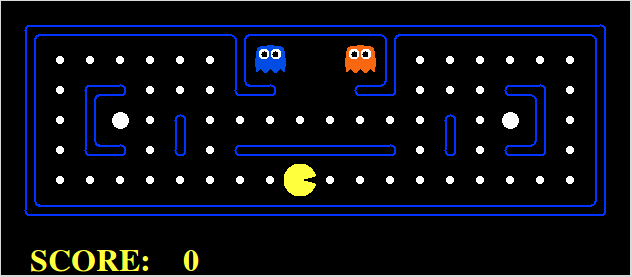
\includegraphics[width=120mm]{images/pacman_small_map}
    \caption{Mapa pequeno do jogo Pacman. Usado nos testes 1 e 3.}
    \label{img:PlataformaPacmanMapaPequeno}
\end{figure}

\subsubsection{Parâmetros Utilizados}

\begin{multicols}{2}

Num. partidas%
\footnote{Número de partidas executadas%
} = 3000;

Num. treinos%
\footnote{Número de partidas usadas para treinamento%
} = 2700;

Num. Greedy%
\footnote{Número de partidas em que foi utilizada exploração gulosa. Como explicado no tópico \ref{subsection:EscolhaDeAçõesExploraçãoGulosa}%
} = 1500;

$ \beta%
\footnote{Fator de exploração gulosa utilizado.%
} = 1 - \left( \frac{n}{Num. Greedy} \right) $;

$ \alpha%
\footnote{Fator de Aprendizagem%
} = 0.002 $;

$ \gamma%
\footnote{Fator de Desconto%
} = 0.99 $;

$ \sigma_{pacman}%
\footnote{Desvio padrão do erro gaussiano da posição recebida do Pacman%
} = 0.5 $;

$ \sigma_{dist\_fant}%
\footnote{Desvio padrão do erro gaussiano da distância recebida para os Fantasmas%
} = 0.5 $;

$ \nu_{atuacao}%
\footnote{Fator de Acerto na movimentação do Pacman. Descrito no algorítmo \ref{algorithm:ErroAtuacao} na seção \ref{section:AmbienteDeTestes}%
} = 0.9 $.

\end{multicols}

Sendo $ n $ o número da partida sendo jogada.

\subsubsection{Comportamentos Utilizados} \label{subsubsection:3ComportamentosUtilizados}

Os comportamentos utilizados foram: parar, comer e fugir. Ou seja:
$$ b \in B = \left\{ Ficar\_Parado, Comer, Fugir \right\}, $$
$$ s_b \in S_b = \left\{ Estado\_Parar, Estado\_Comer, Estado\_Fugir \right\}. $$

Como explicado no tópico \ref{subsection:BayesComSelecaoDeComportamento} agora são usados três modelos de seleção de ação motora: 

\begin{equation}
    P \left( M^t \mid S^t S_b^t M^{t-1} \pi_f \right) = 
        \left\{
            \begin{array}{l}
                P \left( M^t \mid S^t \left[ S_b^t=Estado\_Parar \right] M^{t-1} \pi \right) \\
                P \left( M^t \mid S^t \left[ S_b^t=Estado\_Comer \right] M^{t-1} \pi \right) \\
                P \left( M^t \mid S^t \left[ S_b^t=Estado\_Fugir \right] M^{t-1} \pi \right)
            \end{array}
        \right..
\end{equation}

A seguir, cada modelo é apresentado de forma detalhada.

\subsubsection*{Parar}

Esse é o comportamento mais simples, tendo como modelo de seleção de ação:

\begin{equation}
    P \left( m^t \mid S^t \left[ S_b^t = Estado\_Parar \right] M^{t-1} \pi_f \right) = 
        \left\{
            \begin{array}{l l}
                0.99 & \text{se }m^t = Parar \\
                0.0025 & \text{senão}
            \end{array}
        \right..
\end{equation}

\subsubsection*{Comer}

Para esse comportamento utiliza-se um modelo mais complexo em que, para um dado estado de $ S^t $ se calcula uma ação com o algoritmo \ref{algorithm:SelecaoDeAcaoComer}.

\begin{algorithm}[H]
	\caption{Escolher Ação Comer} \label{algorithm:SelecaoDeAcaoComer}
	\begin{algorithmic}[1]
		\Procedure{Escolher\_Ação\_Comer}{\textit{estado}}
			\State $\textit{pos\_comida} \gets \text{posição }\textit{comida\_mais\_proxima} $
			\State $\textit{pos\_pacman} \gets \text{posição }\textit{pacman} $
			\State $\textit{dist\_atual} \gets \text{dist} \left( \textit{pos\_comida}, \textit{pos\_pacman} \right) $
			\For{Ação $ in $ Ações}
				\State $\textit{nova\_pos\_pacman} \gets \text{executa} \left( \textit{pos\_pacman}, \textit{Ação} \right) $
				\If{$ \text{dist} \left( \textit{pos\_comida}, \textit{nova\_pos\_pacman} \right) < \textit{dist\_atual} $ }
					\State \Return $ \textit{Ação} $
					\Comment{Retorna ação escolhida}
				\EndIf 
			\EndFor
			\State \Return $ \textit{Ação} $
			\Comment{Nenhuma ação boa, mas precisa retornar uma}
		\EndProcedure
	\end{algorithmic}
\end{algorithm}

Depois de calculada essa ação para um estado $ s^t \in S^t $, utiliza-se um modelo parecido com o para o comportamento parado, apresentado na equação \ref{equation:ModeloAcaoComer}.

\begin{equation} \label{equation:ModeloAcaoComer}
    P \left( m^t \mid s^t \left[ S_b^t = Estado\_Comer \right] M^{t-1} \pi_f \right) = 
        \left\{
            \begin{array}{l l}
                0.99 & \text{se }m^t = \textit{Ação} \\
                0.0025 & \text{senão}
            \end{array}
        \right..
\end{equation}

\subsubsection*{Fugir}

Para esse comportamento é utilizado um formato parecido com o de comer, mas com uma escolha de ação diferente. Para um dado estado de $ S^t $ se calcula uma ação usando o algoritmo \ref{algorithm:SelecaoDeAcaoFugir}.

\begin{algorithm}[h]
	\caption{Escolher Ação Fugir} \label{algorithm:SelecaoDeAcaoFugir}
	\begin{algorithmic}[1]
		\Procedure{Escolher\_Ação\_Fugir}{\textit{estado}}
			\State $\textit{pos\_fantasma} \gets \text{posição }\textit{fantasma\_mais\_proximo} $
			\State $\textit{pos\_pacman} \gets \text{posição }\textit{pacman} $
			\State $\textit{dist\_atual} \gets \text{dist} \left( \textit{pos\_fantasma}, \textit{pos\_pacman} \right) $
			\For{Ação $ in $ Ações}
				\State $\textit{nova\_pos\_pacman} \gets \text{executa} \left( \textit{pos\_pacman}, \textit{Ação} \right) $
				\If{$ \text{dist} \left( \textit{pos\_fantasma}, \textit{nova\_pos\_pacman} \right) > \textit{dist\_atual} $ }
					\State \Return $ \textit{Ação} $
					\Comment{Retorna ação escolhida}
				\EndIf 
			\EndFor
			\State \Return $ \textit{Ação} $
			\Comment{Nenhuma ação boa, mas precisa retornar uma}
		\EndProcedure
	\end{algorithmic}
\end{algorithm}

Depois de calculado essa ação para um estado $ s^t \in S^t $, assim como para o comportamento anterior, utiliza-se um modelo parecido com o modelo utilizado pelo comportamento parado.

\begin{equation}
    P \left( m^t \mid s^t \left[ S_b^t = Estado\_Fugir \right] M^{t-1} \pi_f \right) = 
        \left\{
            \begin{array}{l l}
                0.99 & \text{se }m^t = \textit{Ação} \\
                0.0025 & \text{senão}
            \end{array}
        \right.
\end{equation}

\subsubsection{Vetor de Características Utilizado} \label{subsubsection:3ComportamentosVetorCaracterísticas}

\subsubsection*{Bias}

Essa é uma característica que sempre está presente nesse vetor. Ela tem um valor igual a $ 1.0 $ e seu peso $ \omega $ indica quão bom esse comportamento é, independente da situação atual.

$$ f_1 = 1.0 $$

\subsubsection*{Distância para Provável Comida mais Próxima} \label{subsubsection:DistProvavelComida}

Essa característica é proporcional à distância até a posição mais próxima em que é provável existir uma comida. Ela pode ser obtida a partir do algoritmo a seguir:

\begin{algorithm}[H]
	\caption{Obter Característica Distancia Comida} \label{algorithm:ObterCaracteristicaDistanciaComida}
	\begin{algorithmic}[1]
		\Procedure{ObterCaracterísticaDistanciaComida}{\textit{probabilidades\_estados}}
			\State $\textit{max\_prob} \gets 0.0 $
			\For{Posição $ in $ Posições}
				\State $\textit{prob\_comida} \gets \text{probabilidade de comida } \left( \textit{Posição} \right) $
				\If{ $ \textit{prob\_comida} > \textit{max\_prob} $ }
					\State $\textit{max\_prob} \gets \textit{prob\_comida} $
				\EndIf 
			\EndFor
			\For{Posição $ in $ Posições}
				\State $\textit{prob\_comida} \gets \text{probabilidade de comida } \left( \textit{Posição} \right) $
				\If{ $ \textit{prob\_comida} > \frac{\textit{max\_prob} }{2} $ }
					\State $ \text{Prob\_Posições } append \text{ Posição} $
				\EndIf 
			\EndFor
			\State $\textit{pos\_comida} \gets \text{mais proxima }\textit{posição} \in \text{Prob\_Posições} $
			\State $\textit{pos\_pacman} \gets \text{posição }\textit{pacman} $
			\State \Return $ \text{dist} \left( \textit{pos\_comida}, \textit{pos\_pacman} \right)  $
		\EndProcedure
	\end{algorithmic}
\end{algorithm}

Tendo um conjunto de probabilidades $ a \in A $ para os estados:

$$ f_2 = \frac{ObterCaracteristicaDistanciaComida \left( a \right)}{\textit{área\_mapa}} $$

\subsubsection*{Soma das Probabilidades de Fantasmas a menos de 4 Movimentos}

Essa característica é obtida a partir da soma das probabilidades de haver fantasmas a 3 movimentos de distância, ou menos, podendo então ir de $ \left[ 0, num\_fantasmas \cdot 100\% \right] $.

\begin{algorithm}[H]
	\caption{Obter Característica Probabilidades Fantasmas} \label{algorithm:ObterCaracteristicaProbabilidadesFantasmas}
	\begin{algorithmic}[1]
		\Procedure{ObterCaracterísticaProbFantasmas}{\textit{probabilidades\_estados}}
			\State $\textit{total} \gets 0.0 $
			\For{Posição $ in $ Posições}
				\For{Posição2 $ in $ Posições}
					\If{ $ \text{dist} \left( \textit{Posição} , \textit{Posição2} \right) < 4 $ }
						\State $\textit{prob\_pacman} \gets \text{probabilidade pacman } \left( \textit{Posição} \right) $
						\For{Fantasma $ in $ Fantasmas}
							\State $\textit{prob\_fantasma} \gets \text{probabilidade Fantasma } \left( \textit{Posição2} \right) $
							\State $\textit{prob\_normal} \gets \text{probabilidade estar normal } \left( \textit{Fantasma} \right) $
							\Comment{Não branco}
							\State $\textit{total} \gets \textit{total} + \textit{prob\_pacman}  \cdot \textit{prob\_fantasma} \cdot \textit{prob\_normal} $
						\EndFor
					\EndIf
				\EndFor
			\EndFor
			\State \Return $ \textit{total} $
		\EndProcedure
	\end{algorithmic}
\end{algorithm}

$$ f_3 = ObterCaracteristicaProbFantasmas \left( a \right) $$


\subsection{3 Comportamentos no mapa original (Teste 2)} \label{subsection:3ComportamentosMapaOriginal}

Esse teste foi feito no mapa clássico do jogo, mostrado na figura \ref{}, e nele foram utilizados apenas três comportamentos:

\begin{itemize}
	\item Parar
	\item Comer
	\item Fugir
\end{itemize}

\subsubsection{Parâmetros Utilizados}

\begin{multicols}{2}

Num. partidas = 1000

Num. treinos = 700

Num. Greedy = 500

$ \beta = 1 - \left( \frac{n}{Num. Greedy} \right) $

$ \alpha = 0.001 $

$ \gamma = 0.99 $

$ \sigma_{pacman} = 0.5 $

$ \sigma_{dist\_fant} = 0.5 $

$ \nu_{atuacao} = 0.9 $

\end{multicols}

Sendo $ n $ o número da partida sendo jogada.

\subsubsection{Comportamentos Utilizados}

Os comportamentos utilizados foram os mesmos que para o teste anterior e estão descritos no tópico \ref{subsubsection:3ComportamentosUtilizados}.

\subsubsection{Vetor de Características Utilizado}

Para o vetor de características $ f $, foram utilizados parâmetros semelhantes aos do teste anterior, sendo o único diferente o uso da $ \textit{Proximidade para Provável Comida mais Próxima} $ no lugar da $ \textit{Distância para Provável Comida mais Próxima} $.

\subsubsection*{Bias}

$$ f_1 = 1.0 $$

\subsubsection*{Proximidade para Provável Comida mais Próxima}

Essa foi a única característica alterada do teste anterior para esse. Foi utilizada essa proximidade, no lugar da distância, por ter um valor mais alto quando recompensas são recebidas e mais baixo no caso contrário, o que facilita a aprendizagem. Isso pode ser observado na equação \ref{equation:UpdateOmegaQPartiallyObservable}, com um valor $ f_i \left( a, b \right) $ maior, para um mesmo $ erro $, tem-se uma variação maior de $ \omega_i $ ($ \uparrow f_i \rightarrow \uparrow \Delta \omega_i $).

$$ f_2 = \frac{1}{ObterCaracteristicaDistanciaComida \left( a \right) } $$

\subsubsection*{Soma das Probabilidades de Fantasmas a menos de 4 Movimentos}

$$ f_3 = ObterCaracteristicaProbFantasmas \left( a \right) $$

\subsection{5 Comportamentos no mapa pequeno (Teste 3)} \label{subsection:5ComportamentosMapaPequeno}

Esse teste foi feito no mapa pequeno, mostrado na figura \ref{}, e nele foram utilizados todos os cinco comportamentos:

\begin{itemize}
	\item Parar
	\item Comer
	\item Fugir
	\item Comer Cápsula
	\item Caçar
\end{itemize}

\subsubsection{Parâmetros Utilizados}

\begin{multicols}{2}

Num. partidas = 3000

Num. treinos = 2700

Num. Greedy = 1500

$ \beta = 1 - \left( \frac{n}{Num. Greedy} \right) $

$ \alpha = 0.002 $

$ \gamma = 0.99 $

$ \sigma_{pacman} = 0.5 $

$ \sigma_{dist\_fant} = 0.5 $

$ \nu_{atuacao} = 0.9 $

\end{multicols}

Sendo $ n $ o número da partida sendo jogada.


\subsubsection{Comportamentos Utilizados} \label{subsubsection:5ComportamentosUtilizados}

Os comportamentos utilizados foram: parar, comer, fugir, comer cápsula e caçar. Ou seja:
$$ b \in B = \left\{ Ficar\_Parado, Comer, Fugir, Comer\_Capsula, \textit{Caçar} \right\} $$
$$ s_b \in S_b = 
        \left\{
            \begin{array}{l}
                Estado\_Parar, \\
                Estado\_Comer, \\
                Estado\_Fugir, \\
                Estado\_Comer\_Capsula, \\
                \textit{Estado\_Caçar}
            \end{array}
        \right\}
         $$

Como explicado no tópico \ref{subsection:BayesComSelecaoDeComportamento}, e analogamente ao visto para três comportamentos, agora podemos ter cinco modelos de seleção de ação:
\begin{equation}
    P \left( M^t \mid S^t S_b^t M^{t-1} \pi_f \right) = 
        \left\{
            \begin{array}{l}
                P \left( M^t \mid S^t \left[ S_b^t=Estado\_Parar \right] M^{t-1} \pi \right) \\
                P \left( M^t \mid S^t \left[ S_b^t=Estado\_Comer \right] M^{t-1} \pi \right) \\
                P \left( M^t \mid S^t \left[ S_b^t=Estado\_Fugir \right] M^{t-1} \pi \right) \\
                P \left( M^t \mid S^t \left[ S_b^t=Estado\_Comer\_Capsula \right] M^{t-1} \pi \right) \\
                P \left( M^t \mid S^t \left[ S_b^t=\textit{Estado\_Caçar} \right] M^{t-1} \pi \right)
            \end{array}
        \right.
\end{equation}

Os modelos para os estados $ Estado\_Parar $, $ Estado\_Comer $ e $ Estado\_Fugir $ foram os mesmo utilizados no primeiro experimento e estão descritos no tópico \ref{subsubsection:3ComportamentosUtilizados}. Os outros dois modelos, para os estados de comportamento $ Estado\_Comer\_Capsula $ e $ \textit{Estado\_Caçar} $, estão descritos abaixo.

\subsubsection*{Comer Cápsula}

O modelo para o estado $ Estado\_Comer\_Capsula $ é análogo ao do estado $ Estado\_Comer $. Para um dado estado $ s^t \in S^t $ se calculava uma ação com o seguinte algoritmo:

\begin{algorithm}[H]
	\caption{Escolher Ação Comer Cápsula} \label{algorithm:SelecaoDeAcaoComerCápsula}
	\begin{algorithmic}[1]
		\Procedure{EscolherAçãoComerCápsula}{\textit{estado}}
			\State $\textit{pos\_capsula} \gets \text{posição }\textit{capsula\_mais\_proxima} $
			\State $\textit{pos\_pacman} \gets \text{posição }\textit{pacman} $
			\State $\textit{dist\_atual} \gets \text{dist} \left( \textit{pos\_comida}, \textit{pos\_pacman} \right) $
			\For{Ação $ in $ Ações}
				\State $\textit{nova\_pos\_pacman} \gets \text{executa} \left( \textit{pos\_pacman}, \textit{Ação} \right) $
				\If{$ \text{dist} \left( \textit{pos\_capsula}, \textit{nova\_pos\_pacman} \right) < \textit{dist\_atual} $ }
					\State \Return $ \textit{Ação} $
					\Comment{Retorna ação escolhida}
				\EndIf 
			\EndFor
			\State \Return $ \textit{Ação} $
			\Comment{Nenhuma ação boa, mas precisa retornar uma}
		\EndProcedure
	\end{algorithmic}
\end{algorithm}

Depois de calculada essa ação para um estado $ s^t \in S^t $, utilizamos o seguinte modelo probabilístico.

\begin{equation}
    P \left( m^t \mid s^t \left[ S_b^t = Estado\_Comer\_Capsula \right] M^{t-1} \pi_f \right) = 
        \left\{
            \begin{array}{l l}
                0.99 & \text{se }m^t = \textit{Ação} \\
                0.0025 & \text{senão}
            \end{array}
        \right.
\end{equation}


\subsubsection*{Caçar}

O modelo para o estado $ \textit{Estado\_Caçar} $ é análogo ao do estado $ Estado\_Fugir $, só que indo em direção ao fantasma. Para um dado estado $ s^t \in S^t $ se calcula uma ação com o seguinte algoritmo:

\begin{algorithm}[H]
	\caption{Escolher Ação Caçar} \label{algorithm:SelecaoDeAcaoCaçar}
	\begin{algorithmic}[1]
		\Procedure{EscolherAçãoCaçar}{\textit{estado}}
			\State $\textit{pos\_fantasma} \gets \text{posição }\textit{fantasma\_mais\_proximo} $
			\State $\textit{pos\_pacman} \gets \text{posição }\textit{pacman} $
			\State $\textit{dist\_atual} \gets \text{dist} \left( \textit{pos\_fantasma}, \textit{pos\_pacman} \right) $
			\For{Ação $ in $ Ações}
				\State $\textit{nova\_pos\_pacman} \gets \text{executa} \left( \textit{pos\_pacman}, \textit{Ação} \right) $
				\If{$ \text{dist} \left( \textit{pos\_fantasma}, \textit{nova\_pos\_pacman} \right) < \textit{dist\_atual} $ }
					\State \Return $ \textit{Ação} $
					\Comment{Retorna ação escolhida}
				\EndIf 
			\EndFor
			\State \Return $ \textit{Ação} $
			\Comment{Nenhuma ação boa, mas precisa retornar uma}
		\EndProcedure
	\end{algorithmic}
\end{algorithm}

Depois de calculada essa ação para um estado $ s^t \in S^t $, utilizamos o seguinte modelo probabilístico.

\begin{equation}
    P \left( m^t \mid s^t \left[ S_b^t = \textit{Estado\_Caçar} \right] M^{t-1} \pi_f \right) = 
        \left\{
            \begin{array}{l l}
                0.99 & \text{se }m^t = \textit{Ação} \\
                0.0025 & \text{senão}
            \end{array}
        \right.
\end{equation}

\subsubsection{Vetor de Características Utilizado} \label{subsubsection:5ComportamentosVetorCaracterísticas}

O vetor de características $ f $ para esse experimento teve sete parâmetros, sendo 3 deles os usados no experimento anterior (\ref{subsection:3ComportamentosMapaOriginal}) $ Bias $, \textit{Proximidade para Provável Comida mais Próxima} e \textit{Soma das Probabilidades de Fantasmas a menos de 4 Movimentos}. Os outros quatro são:

\begin{itemize}
	\item \textit{Proximidade para Provável Cápsula mais Próxima};
	\item \textit{Probabilidade de ainda Existir uma Cápsula};
	\item \textit{Probabilidade de Existir Fantasma Branco};
	\item \textit{Soma das Probabilidades de Fantasmas Brancos a menos de 4 Movimentos}.
\end{itemize}

Cada um desses experimentos está descrito a seguir.

\subsubsection*{Bias}
$$ f_1 = 1.0 $$

\subsubsection*{Proximidade para Provável Comida mais Próxima}
$$ f_2 = \frac{1}{ObterCaracteristicaDistanciaComida \left( a \right)} $$

\subsubsection*{Proximidade para Provável Cápsula mais Próxima}

Essa característica indica qual a distância até a posição mais próxima em que é provável existir uma cápsula. Ela pode ser obtida a partir do algoritmo a seguir, que é análogo ao algoritmo \ref{algorithm:ObterCaracteristicaDistanciaComida} do tópico \ref{subsubsection:DistProvavelComida}:

\begin{algorithm}[H]
	\caption{Obter Característica Distancia Cápsula} \label{algorithm:ObterCaracteristicaDistanciaCapsula}
	\begin{algorithmic}[1]
		\Procedure{ObterCaracterísticaDistanciaCápsula}{\textit{probabilidades\_estados}}
			\State $\textit{max\_prob} \gets 0.0 $
			\For{Posição $ in $ Posições}
				\State $\textit{prob\_capsula} \gets \text{probabilidade de capsula } \left( \textit{Posição} \right) $
				\If{ $ \textit{prob\_capsula} > \textit{max\_prob} $ }
					\State $\textit{max\_prob} \gets \textit{prob\_capsula} $
				\EndIf 
			\EndFor
			\For{Posição $ in $ Posições}
				\State $\textit{prob\_capsula} \gets \text{probabilidade de capsula } \left( \textit{Posição} \right) $
				\If{ $ \textit{prob\_capsula} > \frac{\textit{max\_prob} }{2} $ }
					\State $ \text{Prob\_Posições } append \text{ Posição} $
				\EndIf 
			\EndFor
			\State $\textit{pos\_capsula} \gets \text{mais proxima }\textit{posição} \in \text{Prob\_Posições} $
			\State $\textit{pos\_pacman} \gets \text{posição }\textit{pacman} $
			\State \Return $ \text{dist} \left( \textit{pos\_capsula}, \textit{pos\_pacman} \right) $
		\EndProcedure
	\end{algorithmic}
\end{algorithm}

Tendo um conjunto de probabilidades $ a \in A $ para os estados:

$$ f_3 = \frac{1}{ObterCaracteristicaDistanciaCapsula \left( a \right)} $$

\subsubsection*{Probabilidade de ainda Existir uma Cápsula}

Essa característica é obtida a partir da probabilidade de ainda existir uma cápsula no mapa.

$$ f_4 = P \left( capsula \mid a \right) $$

\subsubsection*{Probabilidade de Existir Fantasma Branco}

Essa característica é obtida a partir da probabilidade de existir um fantasma branco no ambiente.

$$ f_5 = P \left( fantasma\_branco \mid a \right) $$

\subsubsection*{Soma das Probabilidades de Fantasmas a menos de 4 Movimentos}

$$ f_6 = ObterCaracteristicaProbFantasmas \left( a \right) $$

\subsubsection*{Soma das Probabilidades de Fantasmas Brancos a menos de 4 Movimentos}

Essa característica é obtida a partir da soma das probabilidades de haver fantasmas a 3 movimentos de distância, ou menos, podendo então ir de $ \left[ 0, num\_fantasmas \cdot 100\% \right] $.

\begin{algorithm}[H]
	\caption{Obter Característica Probabilidades Fantasmas Brancos} \label{algorithm:ObterCaracteristicaProbabilidadesFantasmasBrancos}
	\begin{algorithmic}[1]
		\Procedure{ObterCaracterísticaProbFantasmasBrancos}{\textit{probabilidades\_estados}}
			\State $\textit{total} \gets 0.0 $
			\For{Posição $ in $ Posições}
				\For{Posição2 $ in $ Posições}
					\If{ $ \text{dist} \left( \textit{Posição} , \textit{Posição2} \right) < 4 $ }
						\State $\textit{prob\_pacman} \gets \text{probabilidade pacman } \left( \textit{Posição} \right) $
						\For{Fantasma $ in $ Fantasmas}
							\State $\textit{prob\_fantasma} \gets \text{probabilidade Fantasma } \left( \textit{Posição2} \right) $
							\State $\textit{prob\_branco} \gets \text{probabilidade estar branco } \left( \textit{Fantasma} \right) $
							\State $\textit{total} \gets \textit{total} + \textit{prob\_pacman}  \cdot \textit{prob\_fantasma} \cdot \textit{prob\_branco} $
						\EndFor
					\EndIf
				\EndFor
			\EndFor
			\State \Return $ \textit{total} $
		\EndProcedure
	\end{algorithmic}
\end{algorithm}

$$ f_7 = ObterCaracteristicaProbFantasmasBrancos \left( a \right) $$

\subsection{5 Comportamentos no mapa original (Teste 4)} \label{subsection:5ComportamentosMapaOriginal}

Esse teste foi feito no mapa clássico do jogo, mostrado na figura \ref{}, e nele, como no anterior (\ref{subsection:5ComportamentosMapaPequeno}), foram utilizados todos os cinco comportamentos:

\begin{itemize}
	\item Parar
	\item Comer
	\item Fugir
	\item Comer Cápsula
	\item Caçar
\end{itemize}

\subsubsection{Parâmetros Utilizados}

\begin{multicols}{2}

Num. partidas = 1000

Num. treinos = 700

Num. Greedy = 500

$ \beta = 1 - \left( \frac{n}{Num. Greedy} \right) $

$ \alpha = 0.001 $

$ \gamma = 0.99 $

$ \sigma_{pacman} = 0.5 $

$ \sigma_{dist\_fant} = 0.5 $

$ \nu_{atuacao} = 0.9 $

\end{multicols}

Sendo $ n $ o número da partida sendo jogada.


\subsubsection{Comportamentos Utilizados}

Os comportamentos utilizados são os mesmos utilizados no experimento anterior (\ref{subsection:5ComportamentosMapaPequeno}), descritos no tópico \ref{subsubsection:5ComportamentosUtilizados}.

\subsubsection{Vetor de Características Utilizado}

O vetor de características $ f $ usado nesse experimento possui seis características, sendo cinco delas iguais às utilizadas no experimento anterior%
\footnote{Essas características estão melhor descritos no tópico \ref{subsubsection:5ComportamentosVetorCaracterísticas}.%
}. A última é uma combinação das duas restantes \textit{Proximidade para Provável Capsula mais Próxima} e \textit{Probabilidade de ainda Existir uma Capsula} em uma.  O vetor ficou, então, com as seguintes características.

\subsubsection*{Bias}
$$ f_1 = 1.0 $$

\subsubsection*{Proximidade para Provável Comida mais Próxima}
$$ f_2 = \frac{1}{ObterCaracteristicaDistanciaComida \left( a \right)} $$

\subsubsection*{Probabilidade e Proximidade para Provável Cápsula mais Próxima }

Essa é a característica nova inserida para esse experimento e simplifica as duas características anteriores \textit{Proximidade para Provável Capsula mais Próxima} e \textit{Probabilidade de ainda Existir uma Capsula} em uma, sendo o produto das duas.
$$ f_3 = \frac{P \left( capsula \mid a \right)}{ObterCaracteristicaDistanciaCapsula \left( a \right)} $$

\subsubsection*{Probabilidade de Existir Fantasma Branco}
$$ f_4 = P \left( fantasma\_branco \mid a \right) $$

\subsubsection*{Soma das Probabilidades de Fantasmas a menos de 4 Movimentos}
$$ f_5 = ObterCaracteristicaProbFantasmas \left( a \right) $$

\subsubsection*{Soma das Probabilidades de Fantasmas Brancos a menos de 4 Movimentos}
$$ f_6 = ObterCaracteristicaProbFantasmasBrancos \left( a \right) $$



